\section{Target Group}
\begin{figure}[H]
\centering
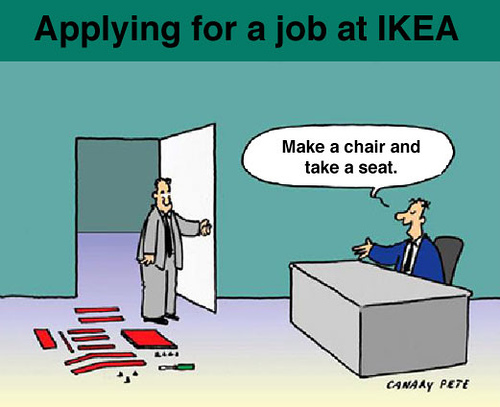
\includegraphics[scale=0.5]{IKEAInterview.jpg}
%\caption{iPhone game using a gyroscope sensor}
\end{figure}
Profound understanding of the target group helps in the process of creating a useful concept. It will be an answer to the users specific needs and wishes. Dividing the target group into different group categorizations - segments, gives a possibility to understand the chosen subjects deeper and hopefully it leads to a better project. The prototype will be specifically designed for a segmented and generalized group of people of this project. Connecting with target group is essential since the product will be used by actual customers. It is not enough to generalize a group of people from surface observations or presumed stereotypes, since sometimes people do not act as they speak and their actual needs can vary a lot. In the target group section, detailed information about the users of IKEA will be revealed.

This project is targeting people who are IKEA customers and who recently started decorating or changing furniture or décor of their home. This section of the research includes two parts - understanding the people who has a need for the application that we develop, and IKEA's target group, the people that IKEA attracts and who are coming to shop for furniture or décor.

There are many ways to segment a target audience. Probably the most popular is Geographic or Demographic segmentation. In this case we will go deeper and have a look at Psychographics too - we want to know the specific needs of the customers which will help to design helpful app. 

\subsection{Demographics }
Demographics is segmenting that describes group of people according age, gender, family size and life cycle (examstutor.com, Demographics). This segment gives a core understanding of the audience and it helps creating other generalizations such as psychographics.

\subsubsection{What is IKEA targeted customer's age ?}
Checking IKEA's report, public documentations, websites -  it is not clear to see what age-range people IKEA is trying to attract. Contacting IKEA also did not result in finding out their specific target group's age-range. According to observations and descriptions of center, IKEA's target group's age-range is really wide - there are lounges for children and considerations for disabled and old people. At "IKEA'S Accessibility Plan" (Accessibility Plan, 2013) they mention that there are consideration to accept people from children to old aged or disabled people. The report even states that the staff is trained to help people with disabilities, their equipment and even their help-animals. All IKEA shops has mini restaurants where different people of varying age can eat. They serve special menus for children, sell wine, and has a quick walk-by coffee machines. An assumption can be made that IKEA is trying to appeal to all age-ranges and has not created a clear concept design around a specific life-cycle stage (examstutor.com, Demographics) nor age range. 
However, according to two interview sessions that were done in a local IKEA center in Copenhagen, it was more clear who is shopping there. The majority of the interviewed people were young people - between 25 and 35 years of age.

\subsubsection{gender}
IKEA does not clearly mention anything about attracting either men or women to shop in public documentation (Accessibility Plan 2013) nor on their website of Ikea.dk. This was also clear to see through observation in IKEA. However it was interesting to see that at least half of the people were shopping together: in pairs, or groups of friends or family. 
\subsubsection{Social-class}
Age and statistical information of Denmark can reveal which life cycle customers of IKEA could belong to. Picture below shows "Life-cycle" stages.
\begin{figure}[H]
\centering
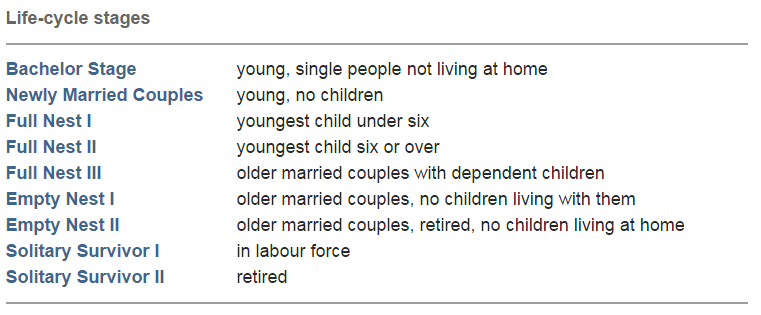
\includegraphics[scale=1]{life_cycle.png}
\caption{Picture from internet -  examtutors.com - demographics}
\end{figure}
The targets group's maximum age was set to 35, according "Statistics denmark" section "The average Dane" women has their first child at the age of 29.(Statistics Denmark 2014 - The Average Dane) This means that the targeted audience is below "Full nest II" - young families. 
 "Danish Ministry of Education" gathered statistical information of when students begin and end their bachelor (Danish Ministry of Education website - Higher education). In the picture below it is seen at which age Danish students start higher education.
\begin{figure}[H]
\centering
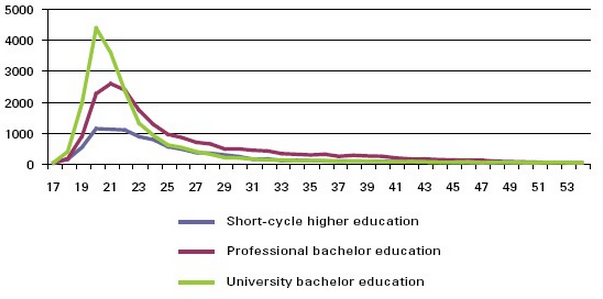
\includegraphics[scale=1]{bachelor.png}
\caption{Picture from internet - Danish Ministry of education - higher education}
\end{figure}
As it is seen in the graph above, students finish their bachelor at around the age of 25. It means that IKEA attracts people who has just finished some higher education and/or continuing master and above, since set minimum was 25.

An assumption can be made that IKEA attracts young people - Higher education students, young couples and families and of course exceptions.

\subsection{Psychographics}
Psychographic generalization segments target group according social class, lifestyle and personality characteristics. (Examstutor.com, Psychographics) It is important and relevant to understand the customer's needs, their habits and personality since it can partially answer how the app's concept can be developed. 
Since IKEA is attracting young - up to middle-aged people, it is possible to do a more accurate analysis of the social class, lifestyle and personality traits of our target group (Examstutor.com,  2015). 
\subsubsection{Economy}
Younger people generally has less money than older generations. As an example, statistical graph from US below shows the difference of income.
\begin{figure}[H]
\centering
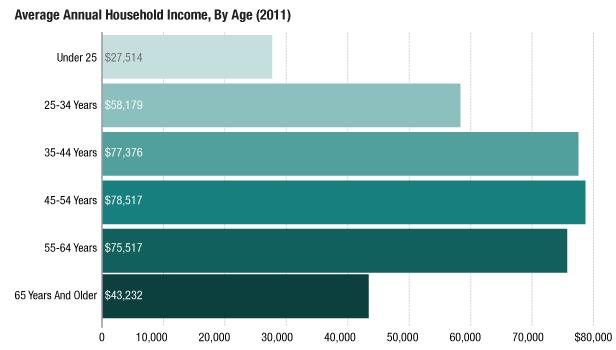
\includegraphics[scale=1]{us_income.jpg}
\caption{Picture from Internet - Income in United States}
\end{figure}

According to the "examstutor" website, social class is categorized in grade class, where IKEA's targeted customers could be defined as class C1, C2, D or E:
\begin{figure}[H]
\centering
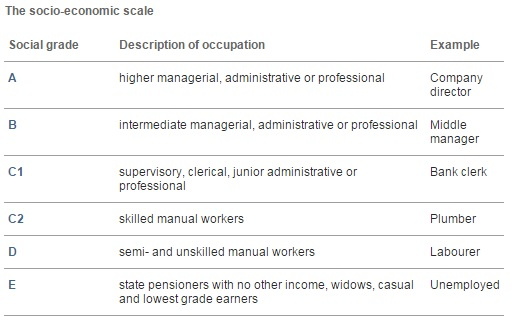
\includegraphics[scale=1]{SocialClassDiagram.jpg}
\caption{Scale of the economic classes}
\end{figure}
People in the lower socio-economic position generally have a lower income. IKEA offers low priced furniture in comparison to other Danish-market shops such as "Silvan", "ILVA" etc - it is easily seen just by visiting the websites of these shops. Therefore an assumption can be made that the younger generation are shopping at IKEA more than other people, because they care more about expenses.  

Interviewing customers confirmed that over half of the participants count their expenses. Furthermore, while interviewing employees of the shop, they noticed that the price is one of the most common topic to talk with customers about. This confirms the social class categorization mentioned above. 

\subsection{Digital knowledge}
Marc Prensky in his "Digital Natives, Digital Immigrants" (Prensky, 2001) article categorizes his understanding of target group into two segments, when it comes to understanding or learning with digital technology. He categorizes them as "digital natives" and "digital immigrants".There are few more categorizations that people use, such as "Born digital" or "Digital Settlers", so it is common to separate people into Idigital knowledge" groups.  Immigrant: Is the one who was born and grew up before the technological revolution, for example a 65 years old man who did not have all the computers and digital tools or equipment that people do now. This person only adopted the technology at a certain age or point in their life when it was needed. Digital native is the one who grew up in the technological era, where he had access for example to the Internet, computers and probably experienced one or more ways of learning in a digital environment (Prensky, 2001). However, Prensky notes that time will make everyone a "digital native", as everyone will be born in a world full of advanced technology, so old generalization terminology will not be suiting in the future. He quotes Albert Einstein - "The problems that exist in the world today cannot be solved by the level of thinking that created them." Prensky later introduces "Digital wisdom" that is a more general term but fitting in this era.(M. Prensky, 2008). This "tag" is best suited to this target group - if IKEA's customers are young students or people around 35 years of age it means that the target group is on the edge of being called both- if a person born in the 80s or 90s he/she had a chance to learn or use modern technology, depending on geographical and social class of course. That is why the terminology of "Digital wisdom" is useful - assumption can be made that most of the target group will be with digital-wisdom. Therefor most of the targeted users should not have huge problems when they start using any digital application.

\subsection{Users do plan}
Interviews with target group also gave knowledge that the users plan and prepare before going to the actual shop. Almost all of the interviewed people do some kind of measurements when buying furniture. All the interviewed people checks the website or catalogue before going to IKEA, the majority do plan before going. 

\subsection{Target group conclusion}
The target group of this project are young - middle aged IKEA customers from 25 to 35 years of age. Almost every customer has access to personal a smartphone and digital-wisdom when it comes to using its applications. The targeted people are careful with their expenses and consider the price, they also tend to know about the product before actually visiting the shop. Excluding exceptions, IKEA's customers are graduated or students who study further than bachelor, also young families and couples.



